\setcounter{page}{1}
\section*{Zielsetzung}

\section{Theorie}
Anhand von Quelle \cite{dem1} werden im Folgenden die relevanten theoretischen Grundlagen zum Thema
Vakuumphysik herausgearbeitet.
\subsection{Definition des Vakuums}
Ein Raum ohne Materie wird Vakuum genannt. Als physikalische Messgröße zur Charakterisierung
des Vakuums wird der \emph{Gasdruck} $p$ verwendet, der durch Stöße von Gasmolekülen mit den Wänden eines Bahälters
entsteht. Da sich in einem Behälter allgemein mehrere Gase befinden, setzt sich der Druck aus der Summe aller
\emph{Partialdrücke} $p\ua{i}$ zusammen.
In Tabelle \ref{tab: vakuumbegriffe} sind Einteilungen des Vakuumbegriffs in Abhängigkeit vom
Druck $p$ aufgeführt.
\begin{table}
  \centering
  \caption{Einteilungen des Vakuumbegriffs in Abhängigkeit vom Gasdruck $p$ \cite{dem1}. Die abgeleitete si-Einheit des Drucks ist
  $[p] = \si{\pascal} = \si{\kilogram \per\meter\per \second\squared}$, es gilt $\SI{1}{\bar} = \SI{e5}{\pascal}$.}
  \label{tab: vakuumbegriffe}
  \begin{tabular}{l l}
    \toprule
    {Vakuumtyp} & {Druckintervall $p/\si{\milli\bar}$} \\
    \midrule
    Grobvakuum &  $[\num{300},\,\num{1}]$ \\
    Feinvakuum &  $(\num{1},\,\num{e-3}]$ \\
    Hochvakuum &  $(\num{e-3},\,\num{e-7}]$ \\
    Ultrahochvakuum &  $(\num{e-7},\,\num{e-12}]$ \\
    \bottomrule
  \end{tabular}
\end{table}
\FloatBarrier Eine weitere wichtige Größe zur Diskussion von Evakuierungsprozessen ist die \emph{mittlere freie
Weglänge} $\Lambda$. Diese ist definiert als die durchschnittliche Länge zwischen zwei Stößen
eines Gasmoleküls. Für eine gemäß Maxwell und Boltzmann verteilte Geschwindigkeit der Gasmoleküle kann
folgende Formel für $\Lambda$ angegeben werden
\begin{equation}
  \Lambda = \frac{1}{\sqrt{2}\pi n D^2}.
\end{equation}
Mit der Stoffmenge $n$ und dem Moleküldurchmesser $D$. Mit fallendem Druck wächst die mittlere freie
Weglänge an und erreicht den theoretischen Wert $\infty$ im idealen Vakuum.

\subsection{Erzeugung des Vakuums}
Eine Apparatur zur Erzeugung eines Vakuums wird als \emph{Vakuumpumpe} bezeichnet. Diese besitzt ein
\emph{Saugvermögen} $S$, das den Gasvolumendurchfluss zwischen Pumpe und \emph{Rezipient}~\footnote{Der Hohlraum, in dem das Vakuum erzeugt werden soll.}
angibt
\begin{equation}
  S = \frac{\dif{}}{\dif{t}} V.
\end{equation}
Das Saugvermögen wird oft bezogen auf das Einheitsvolumen in $[{S}] = \si{\per \second}$ angegeben.
Das Produkt aus Druck $p$ und Saugvermögen $S$ wird als Saugleistung $P\ua{S}$ definiert
\begin{equation}
  P\ua{S} = p S = L \Delta p , \quad [L] = \si{\meter^3 \per \second}.
\end{equation}
Die Saugleistung ist proportional zu einer erzeugten Druckdifferenz $\Delta p$,
wobei der proportionalitätsfaktor $L$ als \emph{Leitwert} bezeichnet wird und stark vom verwendeten Bauteil abhängt.
Der Kehrwert des Leitwertes wird \emph{Strömungswiderstand} $R$ genannt. Der Gesamtsströmungswiderstand einer Leitungsreihe
stellt sich als Summe der einzelnen auftrenden Widerstände dar. Daher gilt für das effektive Saugvermögen $S\ua{eff}$ am Rezipienten
\begin{equation}
 \frac{1}{S\ua{eff}} = \frac{1}{S_0} + \frac{1}{L}.
 \label{eq: effektives_saugvermögen}
\end{equation}
Mit dem Saugvermögen $S_0$ ohne Leitungen (Herstellerangabe).

Der erzeugte Strom durch ein Rohr zwischen Pumpe und Rezipient korreliert mit der mittleren freien Weglänge
und ist damit vom Typ des Vakuums abhängig. Ist $\Lambda$ wesentlich
kleiner als der Durchmesser der verwendeten Bauteile, so kann von \emph{laminaren} bzw. \emph{turbulenten Strömungen} ausgegangen werden. Gilt andersherum
$\Lambda \gg d$, so werden Stöße der Moleküle mit den Wänden relevant.
In diesem Fall wird von einer \emph{molekularen Strömung} gesprochen.


\subsubsection{Vakuumpumpen}
Vakuumpumpen lassen sich in ihrer Funktionsweise in drei Kategorien einteilen: Mechanische Pumpen (z.B. Hubkolbenpumpen,
Drehschieberpumpen, Turbomolekularpumpen), Treibmittelpumpen (z.B. Flüssigkeitsstrahlpumpen, Diffusionspumpen) und
Kondensationspumpen (z.B. Kühlfallen, Kryopumpen). Eine Einordnung der jeweiligen Druckeinsatzbereiche befindet sich in
Abbildung~\ref{fig: einordnung_pumpen}. Im Folgenden sollen die Drehschieberpumpe und die Turbomolekularpumpe
näher vorgestellt werden.

Der Aufbau einer Drehschieberpumpe ist in Abbildung~\ref{fig: drehschieber} schematisch dargestellt. Innherhalb
eines zylinderförmigen Hohlraumes dreht sich ein exzentrisch gelagerter Rotor $R_1$, an dem zwei mit Federn gelagerte
Schieber befestigt sind. Diese haben ständig Kontakt mit der Zylinderwand und sorgen bei Rotation Systems dafür, dass
Gas aus der Saugöffnung $S_1$ komprimiert zum Auslass $A_1$ transportiert wird. Hierdurch entsteht das gewünschte
Druckgefälle zwischen Saugöffnung und Auslass, das zur Evakuierung verwendet werden kann. Mit Drehschieberpumpen
ist es möglich Gleichgewichtsdrücke im Bereich $\num{e-1}$-$\SI{e-3}{\milli\bar}$ zu erzeugen. Ein Nachteil des
Systems liegt in der unvollkommenen Dichtung zwischen Schieber und Zylinderwand. Komplexere Drehschieberpumpen
erreichen bessere Resultate durch mehrstufige Pumpvorgänge, die einen Druckverlust
zwischen Auslass und Saugöffnung minimieren.

Der Rotor einer Turbomolekularpumpe ist in Abbildung~\ref{fig: turbu} zu sehen. Dieser besteht im Wesentlichen aus einer
alternierenden Abfolge von sich drehenden Rotoren und fest montierten Statoren. Die Pumpe nutzt aus, dass die
Desorbtion von Molekülen durch die Bewegung einer Oberfläche im Mittel einen Richtungstrend aufweist. Die Rotorblätter
sind gekippt angebracht. Wird nun ein Gasmolekül von der Rotoroberfläche adsorbiert, so verlässt es die Oberfläche
nach einer gewissen Verweildauer mit einer durch den Rotor erzeugten Geschwindigkeitkomponente nach schäg unten. Hier
wird es von einem Stator aufgefangen und gelangt somit in einen weiter unten gelegenen Rotoreinfangbereich.
Hierdurh entsteht eine Molekularströmung, mit der ein Vakuum erzeugt werden kann. Voraussetzung für den beschriebenen
Effekt ist, dass sich der Rotor so schnell dreht, dass die Moleküle nur an einer Seite der Rotorblätter haften können.
Die hohen Zentrifugalbeschleunigungen erfordern die Verwendung von leichten und gleichzeitig robusten Materialien, wie z.B.
Titan-Aluminium-Legierungen. Mit Turbomolekularpumpen sind Gleihgewichtsdrücke im Bereich von $\num{e-8}$-$\SI{e-9}{\milli\bar}$
zu erreichen.

\begin{figure}
  \centering
  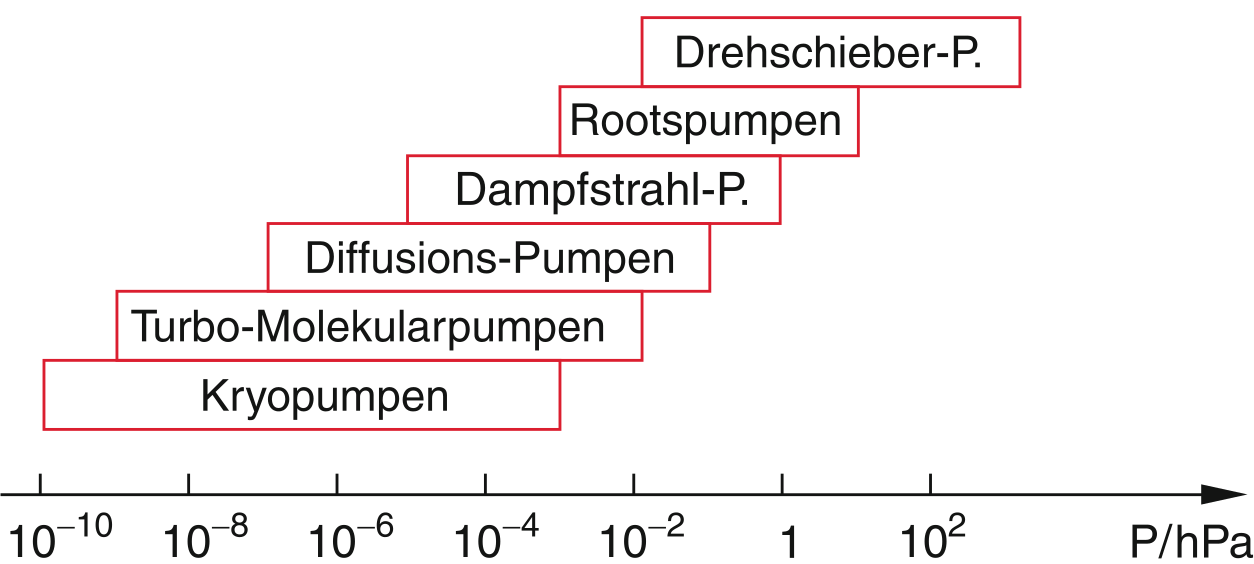
\includegraphics[width = 0.5\textwidth]{theorie_plots/einsatzbereich_pumpen.png}
  \caption{Einsatzbereiche der verschiedenen Pumpentypen in Abhängigkeit des Drucks $P$ \cite{dem1}.}
  \label{fig: einordnung_pumpen}
\end{figure}

\begin{figure}
  \centering
  \begin{subfigure}{0.49\textwidth}
    \centering
    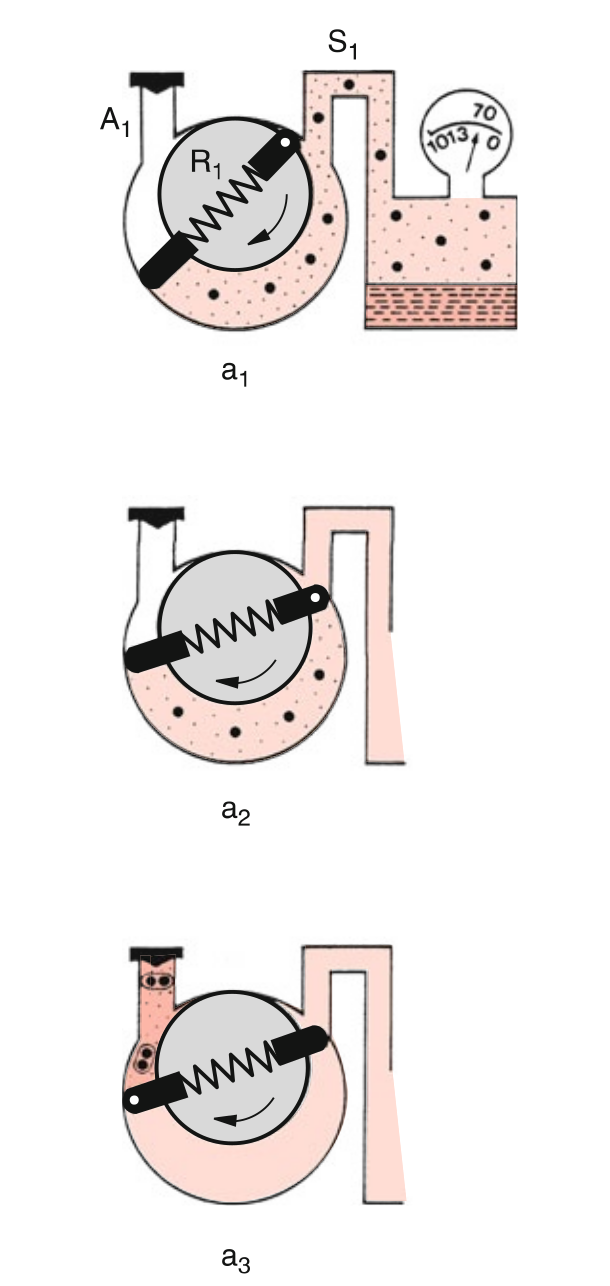
\includegraphics[height = \textwidth]{theorie_plots/drehschieber.png}
    \caption{Funktion der Drehschieberpumpe \cite{dem1}.}
    \label{fig: drehschieber}
\end{subfigure}
\begin{subfigure}{0.49\textwidth}
  \centering
  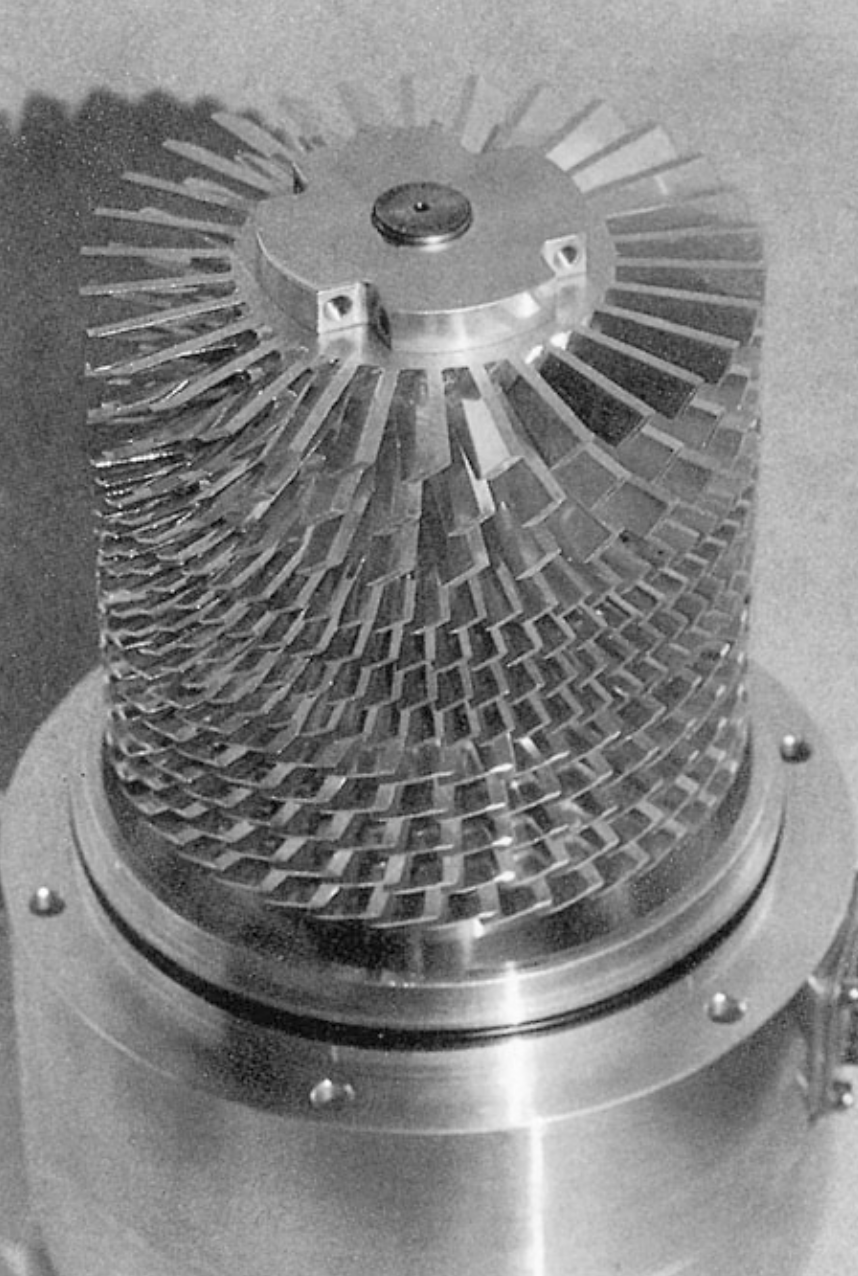
\includegraphics[height = \textwidth]{theorie_plots/turbo_pumpe.png}
  \caption{Rotor einer Turbomolekularpumpe \cite{dem1}.}
  \label{fig: turbo}
\end{subfigure}
\caption{Grafiken zur Erläuterung der Funktionsweise einer Drehschieber und einer Turbomolekularpumpe.}
\label{fig: turbo_drehschieber}
\end{figure}
\FloatBarrier

\subsubsection{Messgeräte}
Zur Druckmessung werden im vorliegenden Versuch ein Ionisationsmannometer nach Bayard-Alpert und ein Penning Vakuummeter verwendet. Eine
alggemeiner Übersicht zu anderen Messgeräten und ihren Einsatzberichen befindet sich in Abbildung \ref{fig: messgeräte}.

Im Ionisationsmannometer werden Elektronen aus einer Glühkathode ausgelöst und mit einer Spannung zu einer Anode beschleunigt.
Im Zwischenraum können sie die
Gasmoleküle des Rezipientengases ionisieren. Ist nun die mittlere freie Weglänge der Elektronen klein gegenüber der
Gesamtbeschleunigerstrecke (kleine Teilchenzahldichte respektive kleiner Druck) so besteht eine direkte Proportionalität
zwischen Anzahl der Ionen und der Teilchendichte und damit ein Zusammenhang zwischen Ionenstrom und Gasdruck.

Das Penning-Vakuummeter verwendet hohe Spannungen zwischen Kathode und Anode, sodass keine Glühemission benötigt wird.
Um die Ionisationswahrscheinlichkeit der Gasmoleküle zwischen Kathode und Anode zu erhöhen werden die Elektronen
durch ein Magnetfeld $B$ auf eine Spiralbahn gelenkt.

\begin{figure}
  \centering
  \includegraphics[width = 0.5\textwidth]{theorie_plots/einsatzbereich_messgeräte.png}
  \caption{Einsatzbereiche der verschiedenen Druckmessgeräte in Abhängigkeit des Drucks $P$ \cite{dem1}.}
  \label{fig: messgeräte}
\end{figure}
\FloatBarrier
\subsection{Zeitlicher Verlauf des Drucks}
Zur Herleitung eines Zusammenhangs für den zeitlichen Verlauf des Drucks $p(t)$, der durch eine Pumpe
hervorgerufen wird, werden im Folgenden einige vereinfachende Annahmen getroffen. Zunächst soll das
verwendete Gas der \emph{idealen Gasgleichung} genügen
\begin{equation}
  p V = n R T.
  \label{eq: ideale_gasgleichung}
\end{equation}
Mit Systemvolumen $V$ und Temperatur $T$. Geht man davon aus, dass das System bestehend aus
Pumpe und Rezipient ideal abgeschlossen ist, so gilt
\begin{equation}
  \frac{\dif{}}{\dif{t}}(n R T ) = 0.
\end{equation}
Und damit das \emph{Boylesche Gesetz}
\begin{equation}
  0 = \dot{p}V  + p\dot{V}.
\end{equation}
Die zeitliche Änderung des Volumens wird als Saugvermögen $S$ der Pumpe angenommen. Es ergibt sich eine Differentialgleichung für $p(t)$
\begin{equation}
  \dot{p} = - \frac{S}{V}\, p,
\end{equation}
die durch Separation der Variablen gelöst werden kann. Zur Zeit $t = 0$ soll der Druck einen Wert $p_0$ haben und für große
Zeiten soll die Funktion gegen einen Grenzwert $p\ua{G} > 0$ laufen. Letzteres wird durch eine Inhomogenität in der DGL berücksichtigt
\begin{equation}
  \dot{p}(t) = - \frac{S}{V} \left(p(t) + p\ua{G}\right).
\end{equation}
Hieraus ergibt sich schließlich
\begin{equation}
  p(t) = (p_0 - p\ua{G})\exp\left(- \frac{S}{V} t \right) + p\ua{G}.
  \label{eq: evakuierungskurve}
\end{equation}
Der Grenzwert $p\ua{G}$ tritt auf, da eine reale Apparatur nicht ideal abgedichtet werden kann.
Eine grafische Darstellung des theoretischen Druckverlaufs $p(t)$ befindet sich in Abbildung~\ref{fig: theo_p_t}.
Über eine Untersuchung von $p(t)$, kann das Saugvermögen mittels
linearer Regression bestimmt werden
\begin{align}
  \begin{aligned}
  \mathup{ln}\left(\frac{p - p\ua{G}}{p_0 - p\ua{G}}\right) &= - \frac{S}{V}\,t = m t \\
  \Leftrightarrow \quad S &= -V m.
  \label{eq: saugvermögen_druckverlauf}
\end{aligned}
\end{align}
\begin{figure}[h]
  \centering
  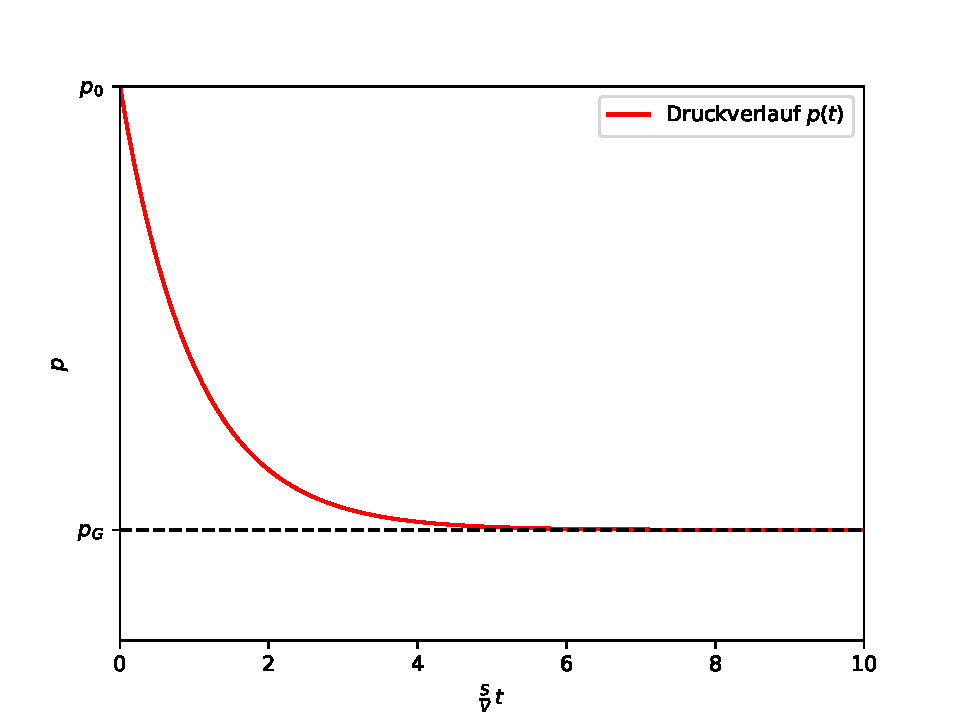
\includegraphics[width = 0.7\textwidth]{theorie_plots/theo_p.pdf}
  \caption{Grafische Darstellung der Funktion $p(t)$ gemäß Gleichung \eqref{eq: evakuierungskurve}.}
  \label{fig: theo_p_t}
\end{figure}
\FloatBarrier
Pro Zeiteinheit
strömt ein Menge an Gas durch auftretende Lecks in den Rezipienten, was analog zur Saugleistung
die Definition einer \emph{Leckrate} $Q$ nahe legt
\begin{equation}
  Q = V \frac{\dif{}}{\dif{t}} p.
\end{equation}
Der Gleichgewichtsdruck stellt sich ein, wenn Leckrate und Saugleistung einander ausgleichen
\begin{equation}
  p\ua{G} S\ua{eff} =  V \frac{\dif{}}{\dif{t}} p \, \Leftrightarrow \,
  S\ua{eff} =  \frac{V}{p\ua{G}} \frac{\dif{}}{\dif{t}} p.
  \label{eq: saugvermögen_leckrate}
\end{equation}
Die Messung der Leckrate ermöglich somit eine weitere Methode zur Bestimmung des effektiven Saugvermögens.
